%!TEX root = ../../Heun_Dale_Haney_A_dynamic_approach_to_input_output_modeling.tex
%%%%%%%%%%%%%%%%%%%%% chapter.tex %%%%%%%%%%%%%%%%%%%%%%%%%%%%%%%%%
%
% sample chapter
%
% Use this file as a template for your own input.
%
%%%%%%%%%%%%%%%%%%%%%%%% Springer-Verlag %%%%%%%%%%%%%%%%%%%%%%%%%%
%\motto{Use the template \emph{chapter.tex} to style the various elements of your chapter content.}

%%%%%%%%%%%%%%%%%%%%%%%%%%%%%%%%%
%%%%%%%%%% Value Flows %%%%%%%%%%
%%%%%%%%%%%%%%%%%%%%%%%%%%%%%%%%%
\chapter{Value flows}
\label{chap:value} % Always give a unique label
% use \chaptermark{}
% to alter or adjust the chapter heading in the running head
\chaptermark{Value}
%%%%%%%%%%%%%%%%%%%%%%%%%%%%%%%%%
%%%%%%%%%%%%%%%%%%%%%%%%%%%%%%%%%
%%%%%%%%%%%%%%%%%%%%%%%%%%%%%%%%%




\abstract*{[NEED TO ADD ABSTRACT HERE]}

%% \abstract{Each chapter should be preceded by an abstract (10--15 lines long) that summarizes the content. The abstract will appear \textit{online} at \url{www.SpringerLink.com} and be available with unrestricted access. This allows unregistered users to read the abstract as a teaser for the complete chapter. As a general rule the abstracts will not appear in the printed version of your book unless it is the style of your particular book or that of the series to which your book belongs.\newline\indent
%% Please use the 'starred' version of the new Springer \texttt{abstract} command for typesetting the text of the online abstracts (cf. source file of this chapter template \texttt{abstract}) and include them with the source files of your manuscript. Use the plain \texttt{abstract} command if the abstract is also to appear in the printed version of the book.}

%% Use the template \emph{chapter.tex} together with the Springer document class SVMono (monograph-type books) or SVMult (edited books) to style the various elements of your chapter content in the Springer layout.


In Chapters~\ref{chap:direct_energy} and~\ref{chap:embodied_energy}, 
we noted that energy is the currency of Thermodynamics,
and we developed accounting equations for flows of 
direct ($\dot{E}$) and embodied ($\dot{B}$) energy through an economy.
In this chapter, we develop a framework for accounting
value flows\index{economic value!flow of} ($\dot{X}$) through economies.
Accounting flows of value is a necessary step along
the path to developing equations (in Chapter~\ref{chap:intensity}) 
that describe the energy intensity of intermediate
and final products within an economy.


%%%%%%%%%% Methodology %%%%%%%%%%
\section{Methodology}
\label{sec:Value_Methodology}
%%%%%%%%%%
We begin by explicitly describing what we mean by value. 
We follow the standard, neoclassical approach of using the market price at the time of an exchange
 to determine the value of the flows of products (goods, services and capital). 

We note, however, that the neoclassical approach is a subjective theory of value. 
It is determined by the relative ability of the product to satisfy a person’s wants. 
A person’s wants are malleable and are, in turn, formed within a ``constellation of shared goals to which a society aspires.’’ ~\cite{costanza2004}
 Thoughout history, economists (particularly the classicals) and non-economists have searched for an invariant, objective, 
intrinsic determinant of value.~\footnote{Following the ecological economics literature, we use the term, intrinsic, in the sense of “objective.” Costanza ~\cite{costanza2004} 
notes that a better term would be objective in order to avoid moral overtones associated with the term intrinsic. } 
Adam Smith, Karl Marx, David Ricardo and his student Sraffa all proposed alternative determinants of value.  
Their proposed objective values were based on identifying the primary input into production,
 such as labor or land and using that input in the sense of a numeraire. 
That is, a way to measure value across the entire spectrum of goods and services in commensurate units.

Costanza ~\cite{costanza2004} makes a compelling case for energy as the only truly primary input into production 
and thus an, or rather the, objective determinant of value. On a global scale, he notes, (solar) energy 
(including that which is stored in fossil fuels) is the only primary input into production, everything else is an intermediate input. 
Thus, free energy could be seen as not simply an input into production, but the primary input into production, upon which an objective (intrinsic), energy theory of value could be built. In fact, this line of research has yielded some interesting figures on the amount of solar energy
 required to run the economy. See Section~\ref{sec:emergy} for further discussion.

It is important to be clear that despite our focus on material and energy flows through an economy, 
our framework does not assume, nor does it lead to an energy theory of value. 
We are working within the neoclassical framework and using an subjective theory of value. 
That is, the goods and services are valued based on market transactions. We do so to attempt to bridge the gap between neoclassical and ecological economics. 

Because the basic unit of analysis in our framework is the economic sector, 
flows of value within the economy are based on the prices agreed for transactions that occur among economic sectors within the economy. 
The flows of value that accompany the material and energy flows in and out of one sector in an economy are depicted in~\ref{fig:basic_value}. 


\begin{figure}[!ht]
\centering
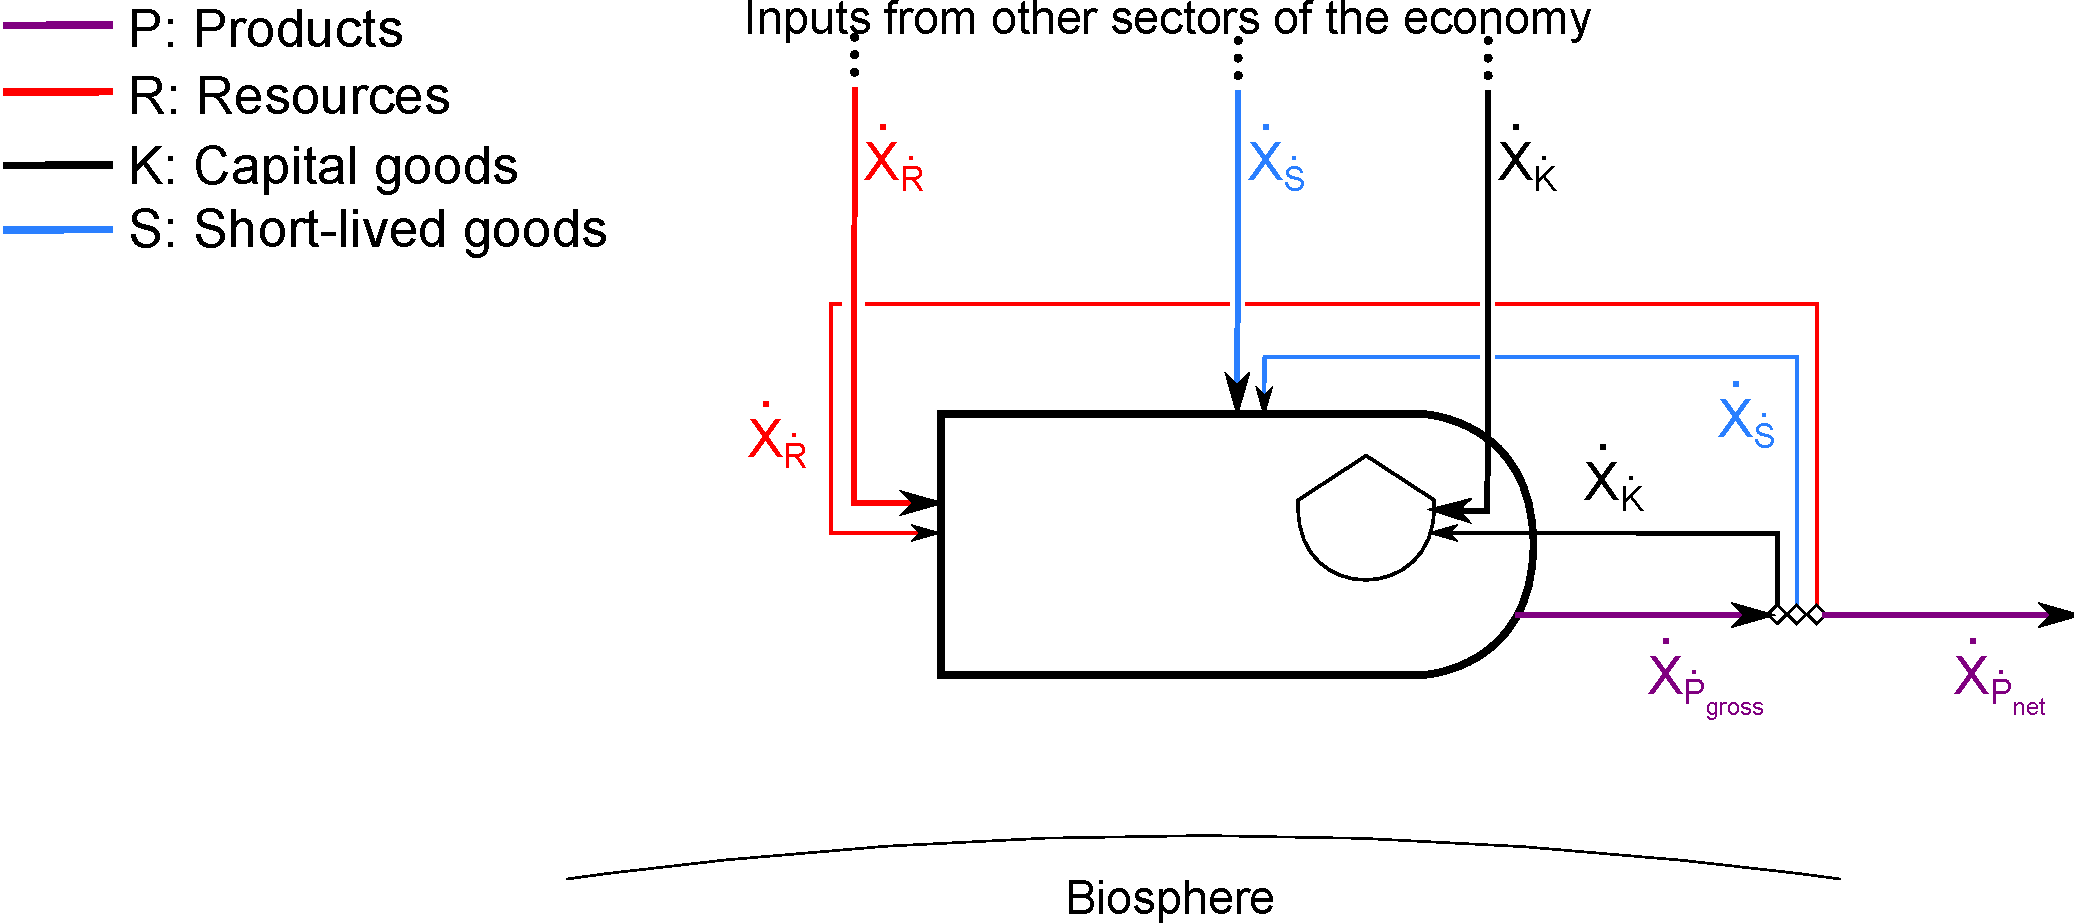
\includegraphics[width=0.8\linewidth]{Part_2/Chapter_Values/images/PERKS_basic_unit_value_all.pdf}
\caption[Flows of value for a single sector]{Flows of value ($\dot{X}$) 
for a single sector. 
The value flows are associated with each of the different 
material and energy flows outlined in previous chapters.}
\label{fig:basic_value} 
\end{figure}

The neoclassical approach measures ``value-added,’’ the value of the products that is greater than the value of the inputs.
 In ~\ref{fig:basic_value_aggregated}, the open circle, ``source,’’ inside the economic sector represents the value-added,
 that is, the value that is created by the economic processes within that sector. 
The flows of value from a value-source are denoted $\dot{X}_{gen}$. 
Similarly, black circles represent the value ``sinks’’  where value is destroyed by economic  processes or natural disasters. 
The flows of value into the value sinks are denoted $\dot{X}_{dest}$. 
Although we do not define the value creation and destruction processes any further (mathematically), we discuss what is meant by the
underlying processes in more detail below.


\begin{figure}[!ht]
\centering
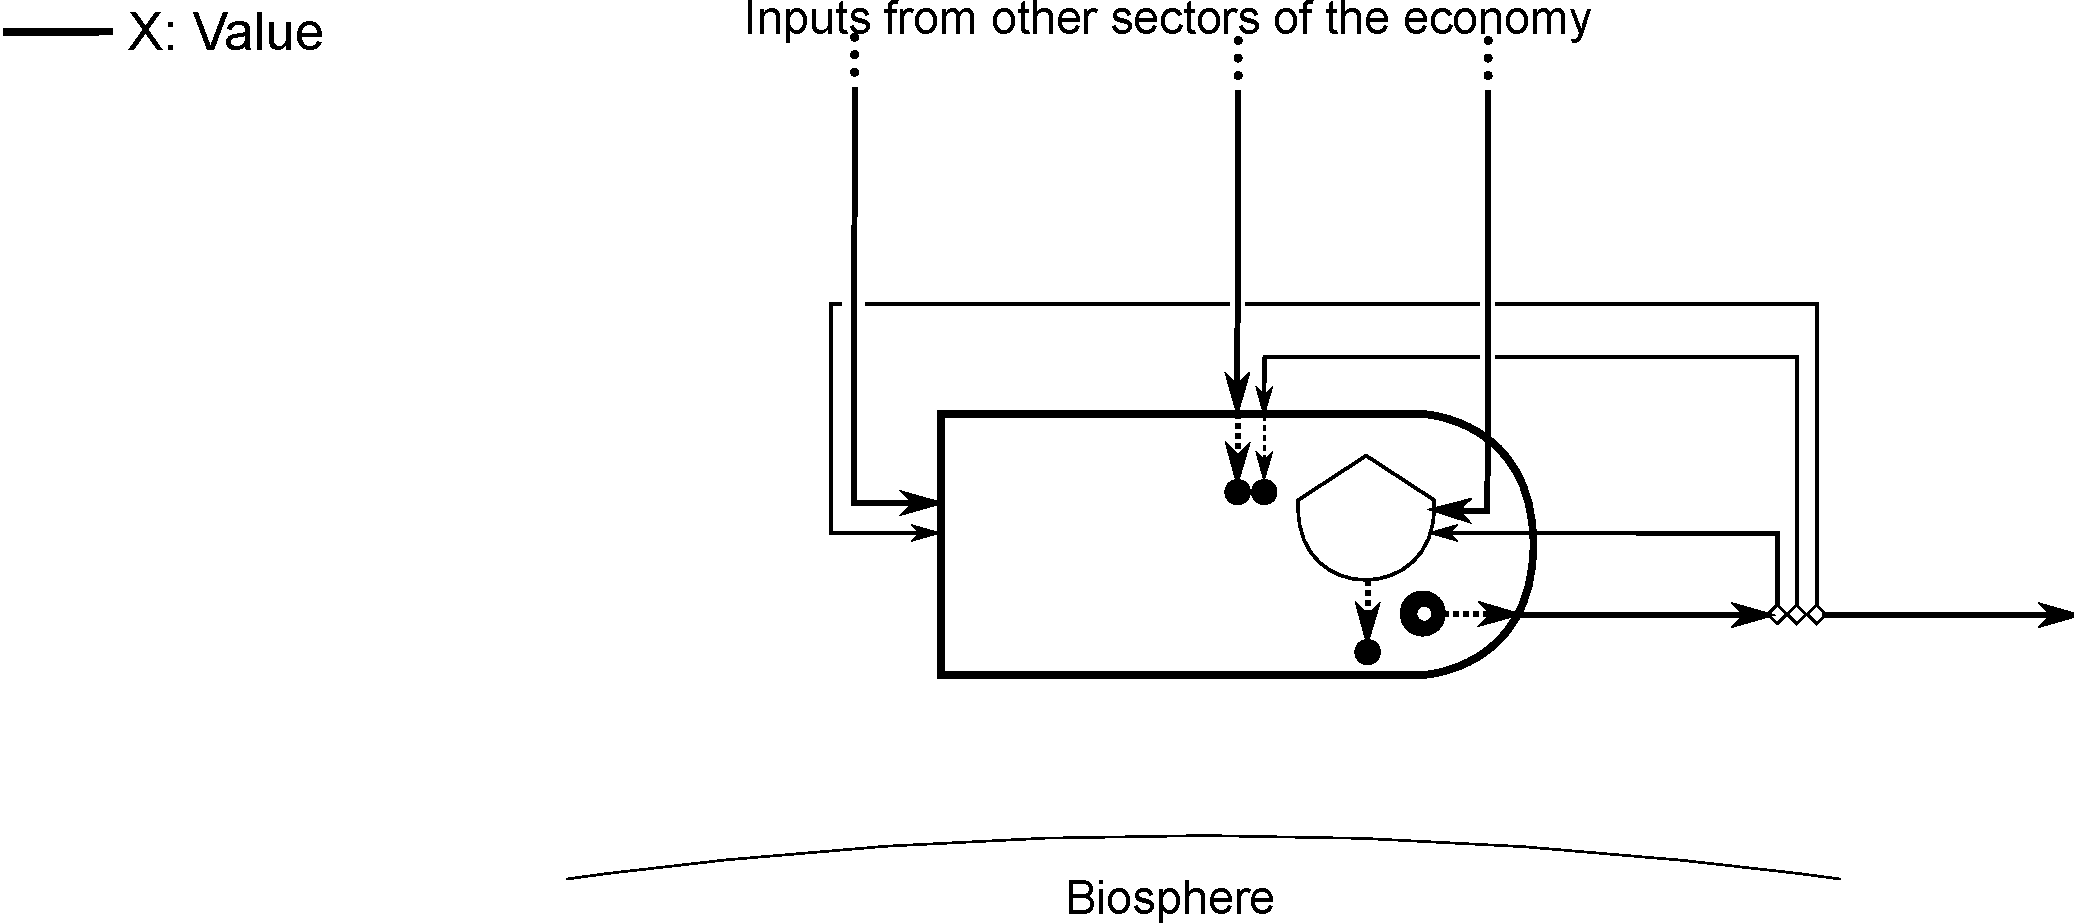
\includegraphics[width=0.8\linewidth]{Part_2/Chapter_Values/images/PERKS_basic_unit_value.pdf}
\caption[Aggregated flows of value for a single sector]{Aggregated flows of value ($\dot{X}$) 
for a single sector. 
Distinction is made between value flows that 
enter the sector and are accumulated (i.e.\ capital goods) 
and value flows that are not accumulated. 
Within the sector there is destruction of value $\dot{X}_{dest}$, 
represented by the downward arrow flowing 
into the black sink and generation of value, 
represented by the arrow flowing out of a source. }
\label{fig:basic_value_aggregated} 
\end{figure}


Herman Daly~\cite{daly1995} provides an overlooked, but important discussion of the measurement of ``value-added.’’
 Standard economic models tend to focus on the value that is added by human processes for human needs and
the value-added provided by natural processes are ignored. The neoclassical framework focuses on measuring value-added and not measuring what the value is added \emph{to}.
Again, this is highlighted by the lack of value flows to and from the biosphere in standard models. 

While we do not attempt to correct this widely utilized approach, 
we note that our model provides a natural framework for including value flows to and from the biosphere. 
Once general principles are agreed to on how to quantify the value of those flows, 
we could reconnect the economy to the biosphere as in~\ref{fig:basic_value_with_biosphere_flows}.~\footnote{As of this printing, the System of Environmental-Economic Accounting (SEEA) is in its third revision using a process of global consultation. 
This system contains internationally agreed-upon standards for quantifying value flows to and from the biosphere. 
This is a system analogous to the System of National Accounts (SNA) which counts economic value flows. 
More information can be found at http://unstats.un.org/unsd/envaccounting/seea.asp.}


 **** MIK - can you create a fig. 5.3 -- that would add in 0j and j0 value flows as dashed lines? (I referred to it with label  basic\_value\_with\_biosphere\_flows)****

****BRH to flesh out further: Daly and Costanza distinguishes between scale, allocation \& distribution -- 
	what scale -- throughput of materials -- is viable for the biosphere to handle
	how should the common wealth be distributed
	only then can you let the market work -- within set boundaries****


%%%%%%%%%% Example A: single-sector economy %%%%%%%%%%
\section{Example A: single-sector economy} % chktex 13
%%%%%%%%%%

Figure~\ref{fig:A_value} shows flows of value in the single-sector economy.
Following typical assumptions in economic modeling, 
the economy is \emph{completely isolated} from the biosphere
in terms of both material inputs and wastes.
In other words, the value flows of an economy are \emph{independent from}
material inputs and wastes.
Value flows are independent from material inputs,
because raw materials have no economic value 
until they have been removed from the biosphere by the extraction industry.
Value flows are independent from wastes,
because wastes, by definition, have no economic value 
after they leave the economy.

\begin{figure}[!ht]
\centering
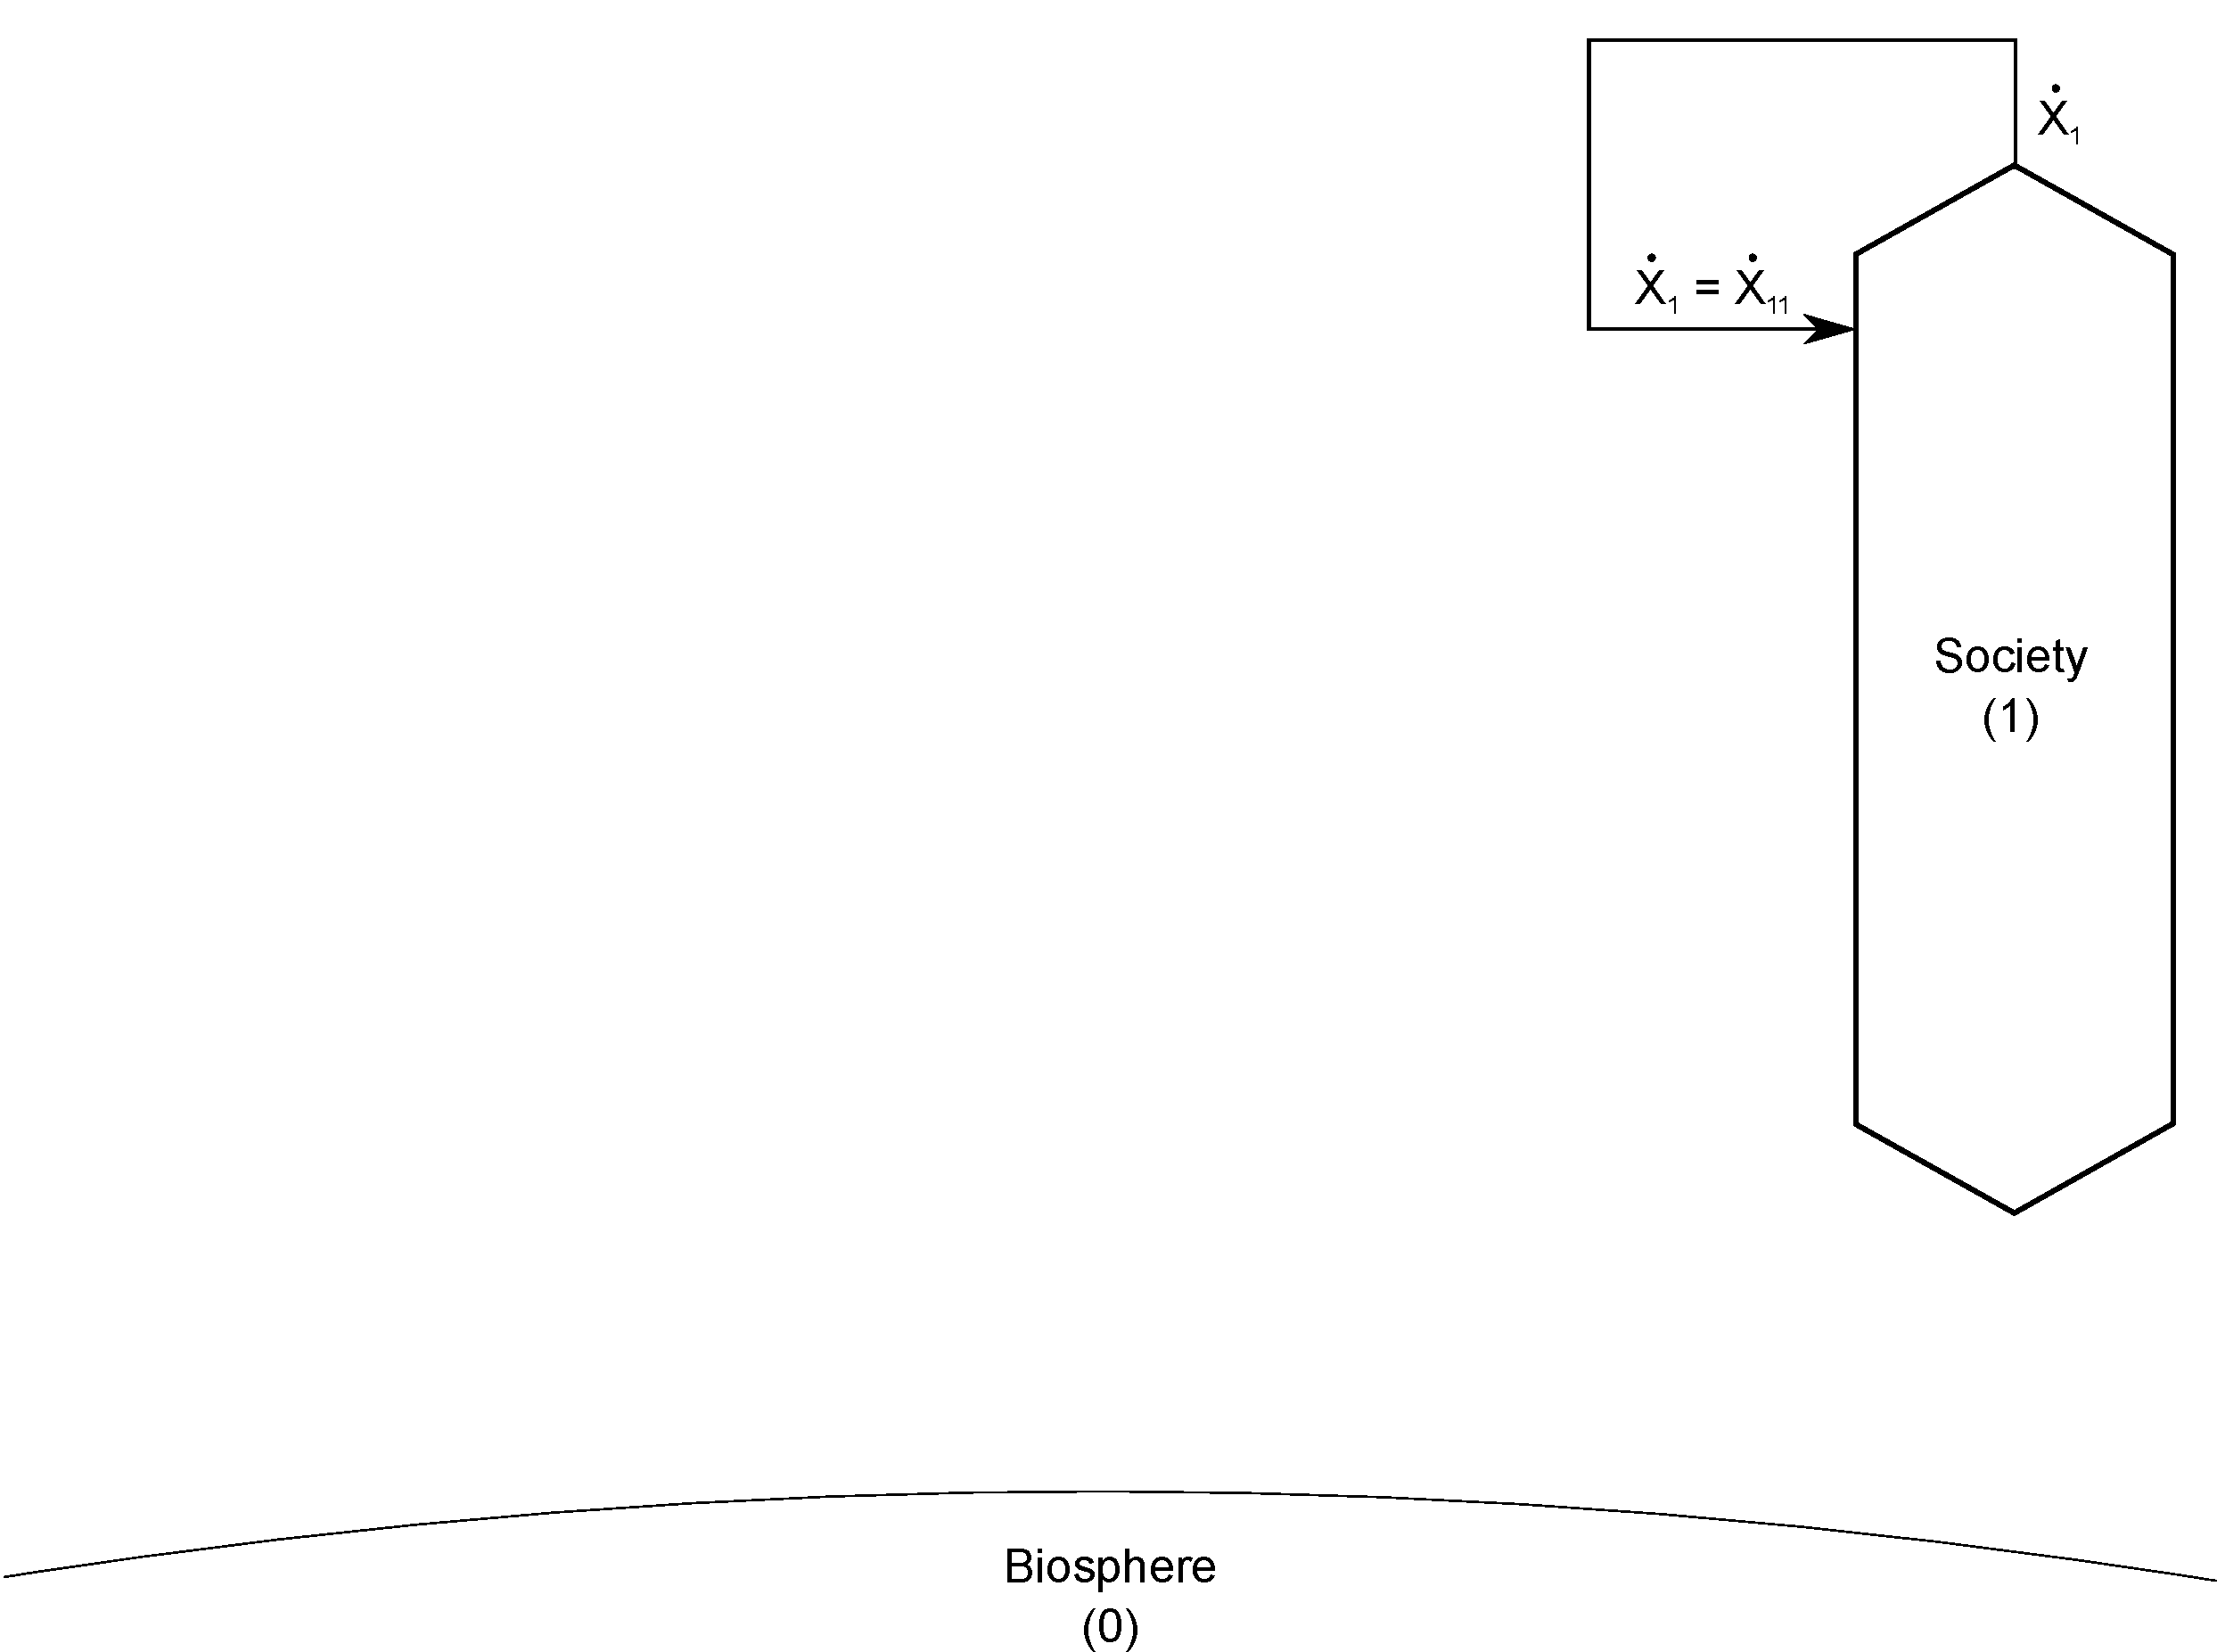
\includegraphics[width=0.8\linewidth]{Part_2/Chapter_Values/images/1_sector_value.pdf}
\caption[Flows of value for a one-sector economy]{Flows of value ($\dot{X}$) for a one-sector economy.}
\label{fig:A_value} 
\end{figure}

The contrast between Figures~\ref{fig:A_materials} and~\ref{fig:A_energy}, 
on the one hand, 
and Figure~\ref{fig:A_value}, 
on the other, is striking.  
The picture of material and energy flows in 
Figures~\ref{fig:A_materials} and~\ref{fig:A_energy} 
indicates a dependence upon the biosphere 
that is not reflected in the value flows of Figure~\ref{fig:A_value}.
The isloation of the value flows from the biosphere is a consequence
of the subjective theory of value\index{theory of value!subjective} 
that underpins modern economics.
The biosphere is akin to a third party with no voice 
in determining the value of a transaction:
it is neither buyer nor seller. 

Equation~\ref{eq:A_X_acct_1} describes the accumulation 
of value\index{economic value!accumulation}
($X$)\nomenclature[X]{$X$}{stock of economic value [\$]} in Society (1).

\begin{equation} \label{eq:A_X_acct_1}
	\frac{\mathrm{d}X_{1}}{\mathrm{d}t} 
	= \dot{X}_{11} 
	- \dot{X}_{1}
	+ \dot{X}_{gen,1}
	- \dot{X}_{dest,1}.
\end{equation}
\nomenclature[X]{$\dot{X}$}{economic value flow rate [\$/s]}
\nomenclature[Xgen]{$\dot{X}_{gen}$}{rate of generation of economic value [\$/s]}
\nomenclature[Xdest]{$\dot{X}_{dest}$}{rate of destruction of economic value [\$/s]}

\noindent{} The following subsections discuss the terms in Equation~\ref{eq:A_X_acct_1}.


%+++++++++ Example A: Economic Transactions ++++++++++
\subsection{Economic transactions ($\dot{X}_{11}$ and $\dot{X}_{1}$)}
%+++++++++

The returning arrow in Figure~\ref{fig:A_value} 
represents transactions between 
\begin{itemize}
	\item{buyers (who receive things of value, $\dot{X}_{11}$,
	in exchange for currency) and}
	\item{sellers (who give up things of value, $\dot{X}_{1}$,
	in exchange for currency).}
\end{itemize}

It is interesting to note that when a good is sold for more
than the producer paid for its inputs, 
the seller has created value and sold it into the economy. 
As a consequence, the seller's stock of currency grows,
providing the seller with an increased level of claim 
on value in the economy.

The subjective theory of value\index{theory of value!subjective}
(Section~\ref{sec:Value_Methodology})
posits that buyers and sellers agree on value at the 
time of the transaction.
Thus, $\dot{X}_{1} = \dot{X}_{11}$, and Equation~\ref{eq:A_X_acct_1}
simplifies to

\begin{equation} \label{eq:A_X_acct_2}	
	\frac{\mathrm{d}X_{1}}{\mathrm{d}t}	
	= \dot{X}_{gen,1}
	- \dot{X}_{dest,1},
\end{equation}

\noindent{}indicating that value accumulates in the economy
$\left( \frac{\mathrm{d}X_{1}}{\mathrm{d}t} \right)$
due to value generation ($\dot{X}_{gen,1}$) 
and destruction ($\dot{X}_{dest,1}$) processes only.


%+++++++++ Example A: value generation ++++++++++
\subsection{Value generation ($\dot{X}_{gen}$)}
%+++++++++

\noindent In Equation~\ref{eq:A_X_acct_1}, 
the value generation term ($\dot{X}_{gen}$) is akin to growing apples
in Section~\ref{sec:Materials_Methodology}: 
value is generated, seemingly out of nothing.
But, in fact, value is not created out of nothing. 
Rather, value is created from a variety of factors that have no apparent 
monetary cost to producers, including:

\begin{itemize}
	\item{flow of solar energy\index{solar energy}\index{energy!solar|see{solar energy}}
	into the economy,
	as in the example of growing apples,}
	\item{extraction of resources (e.g., water\index{water}, minerals\index{minerals}, and
	fossil fuels\index{fossil fuels}) or any other unpriced goods from the biosphere,}
	\item{exploitation of the unpriced waste assimilation capacity of the biosphere,}
	\item{utilization of capital stock, labor, and energy to produce products
	that are more valuable than inputs, and}
	\item{application of human ingenuity\index{ingenuity!human} 
	and innovation\index{innovation}, 
	which lead to increasingly efficient production processes.}
\end{itemize}

\noindent{}The subjective theory of value indicates that 
there is no economic value associated with these ``transactions''
that generate value, because no currency is exchanged. 

The above factors indicate that the process of value generation
has both direct and indirect impacts on the biosphere.
The direct impacts are obvious: 
extraction of non-renewable resources from the biosphere, 
at rates greater than their natural accretion,
represents unsustainable overuse of natural capital.
The indirect impacts are less obvious: 
human ingenuity can lead to increased wealth,
leading to increased demand rates for goods and services, 
whose production requires ever-increasing rates 
of unsustainable natural resource extraction.

$\dot{X}_{gen}$ is accounted as ``value added'' to an industry in the BEA tables.
**** Becky: is this correct? 
Becky: look at the BEA tables' definition of ``value added'' to 
see if there is another sentence that can be added for clarification. ****


%+++++++++ Example A: value destruction ++++++++++
\subsection{Value destruction ($\dot{X}_{dest}$)}
%+++++++++

\noindent In Equation~\ref{eq:A_X_acct_1}, 
the value destruction term ($\dot{X}_{dest}$)\index{economic value!destruction of} 
is akin to consuming apples: 
value is destroyed by a process that consumes, 
or otherwise renders unusable, 
previously-valuable things in the economy
(see Section~\ref{sec:Materials_Methodology}).
The factors that lead to value destruction
($\dot{X}_{dest}$) include:

\begin{itemize}
	\item{depreciation\index{depreciation}, usually associated with disposal of 
	materials and equipment to the biosphere at end of life and}
	\item{natural disasters, such as hurricanes and typhoons,
	that destroy equipment and property.}
\end{itemize}

$\dot{X}_{dest}$ is accounted as **** what **** to an industry in the BEA tables.
Is it simply a negative ``value add?''
**** Becky: What do we write here? ****


%+++++++++ Example A: GDP and Stock of Value ++++++++++
\subsection{GDP and the stock of value}
%+++++++++

If Society (1) in Figure~\ref{fig:A_value} represents 
the economy of an entire country, 
$\dot{X}_{1}$ is its gross domestic product (GDP)\index{gross domestic product}
in units of \$/year.
The stock of value, $X_1$, is the total value of everything that 
is accumulated in society.

**** Becky: anything to add to the above sections? ****


%%%%%%%%%% Example B: two-sector economy %%%%%%%%%%
\section{Example B: two-sector economy} % chktex 13
%%%%%%%%%%

Figure~\ref{fig:B_value} shows flows of value ($\dot{X}$) 
within a two-sector economy. 
Again, we note the isloation of value from the biosphere.

\begin{figure}[!ht]
\centering
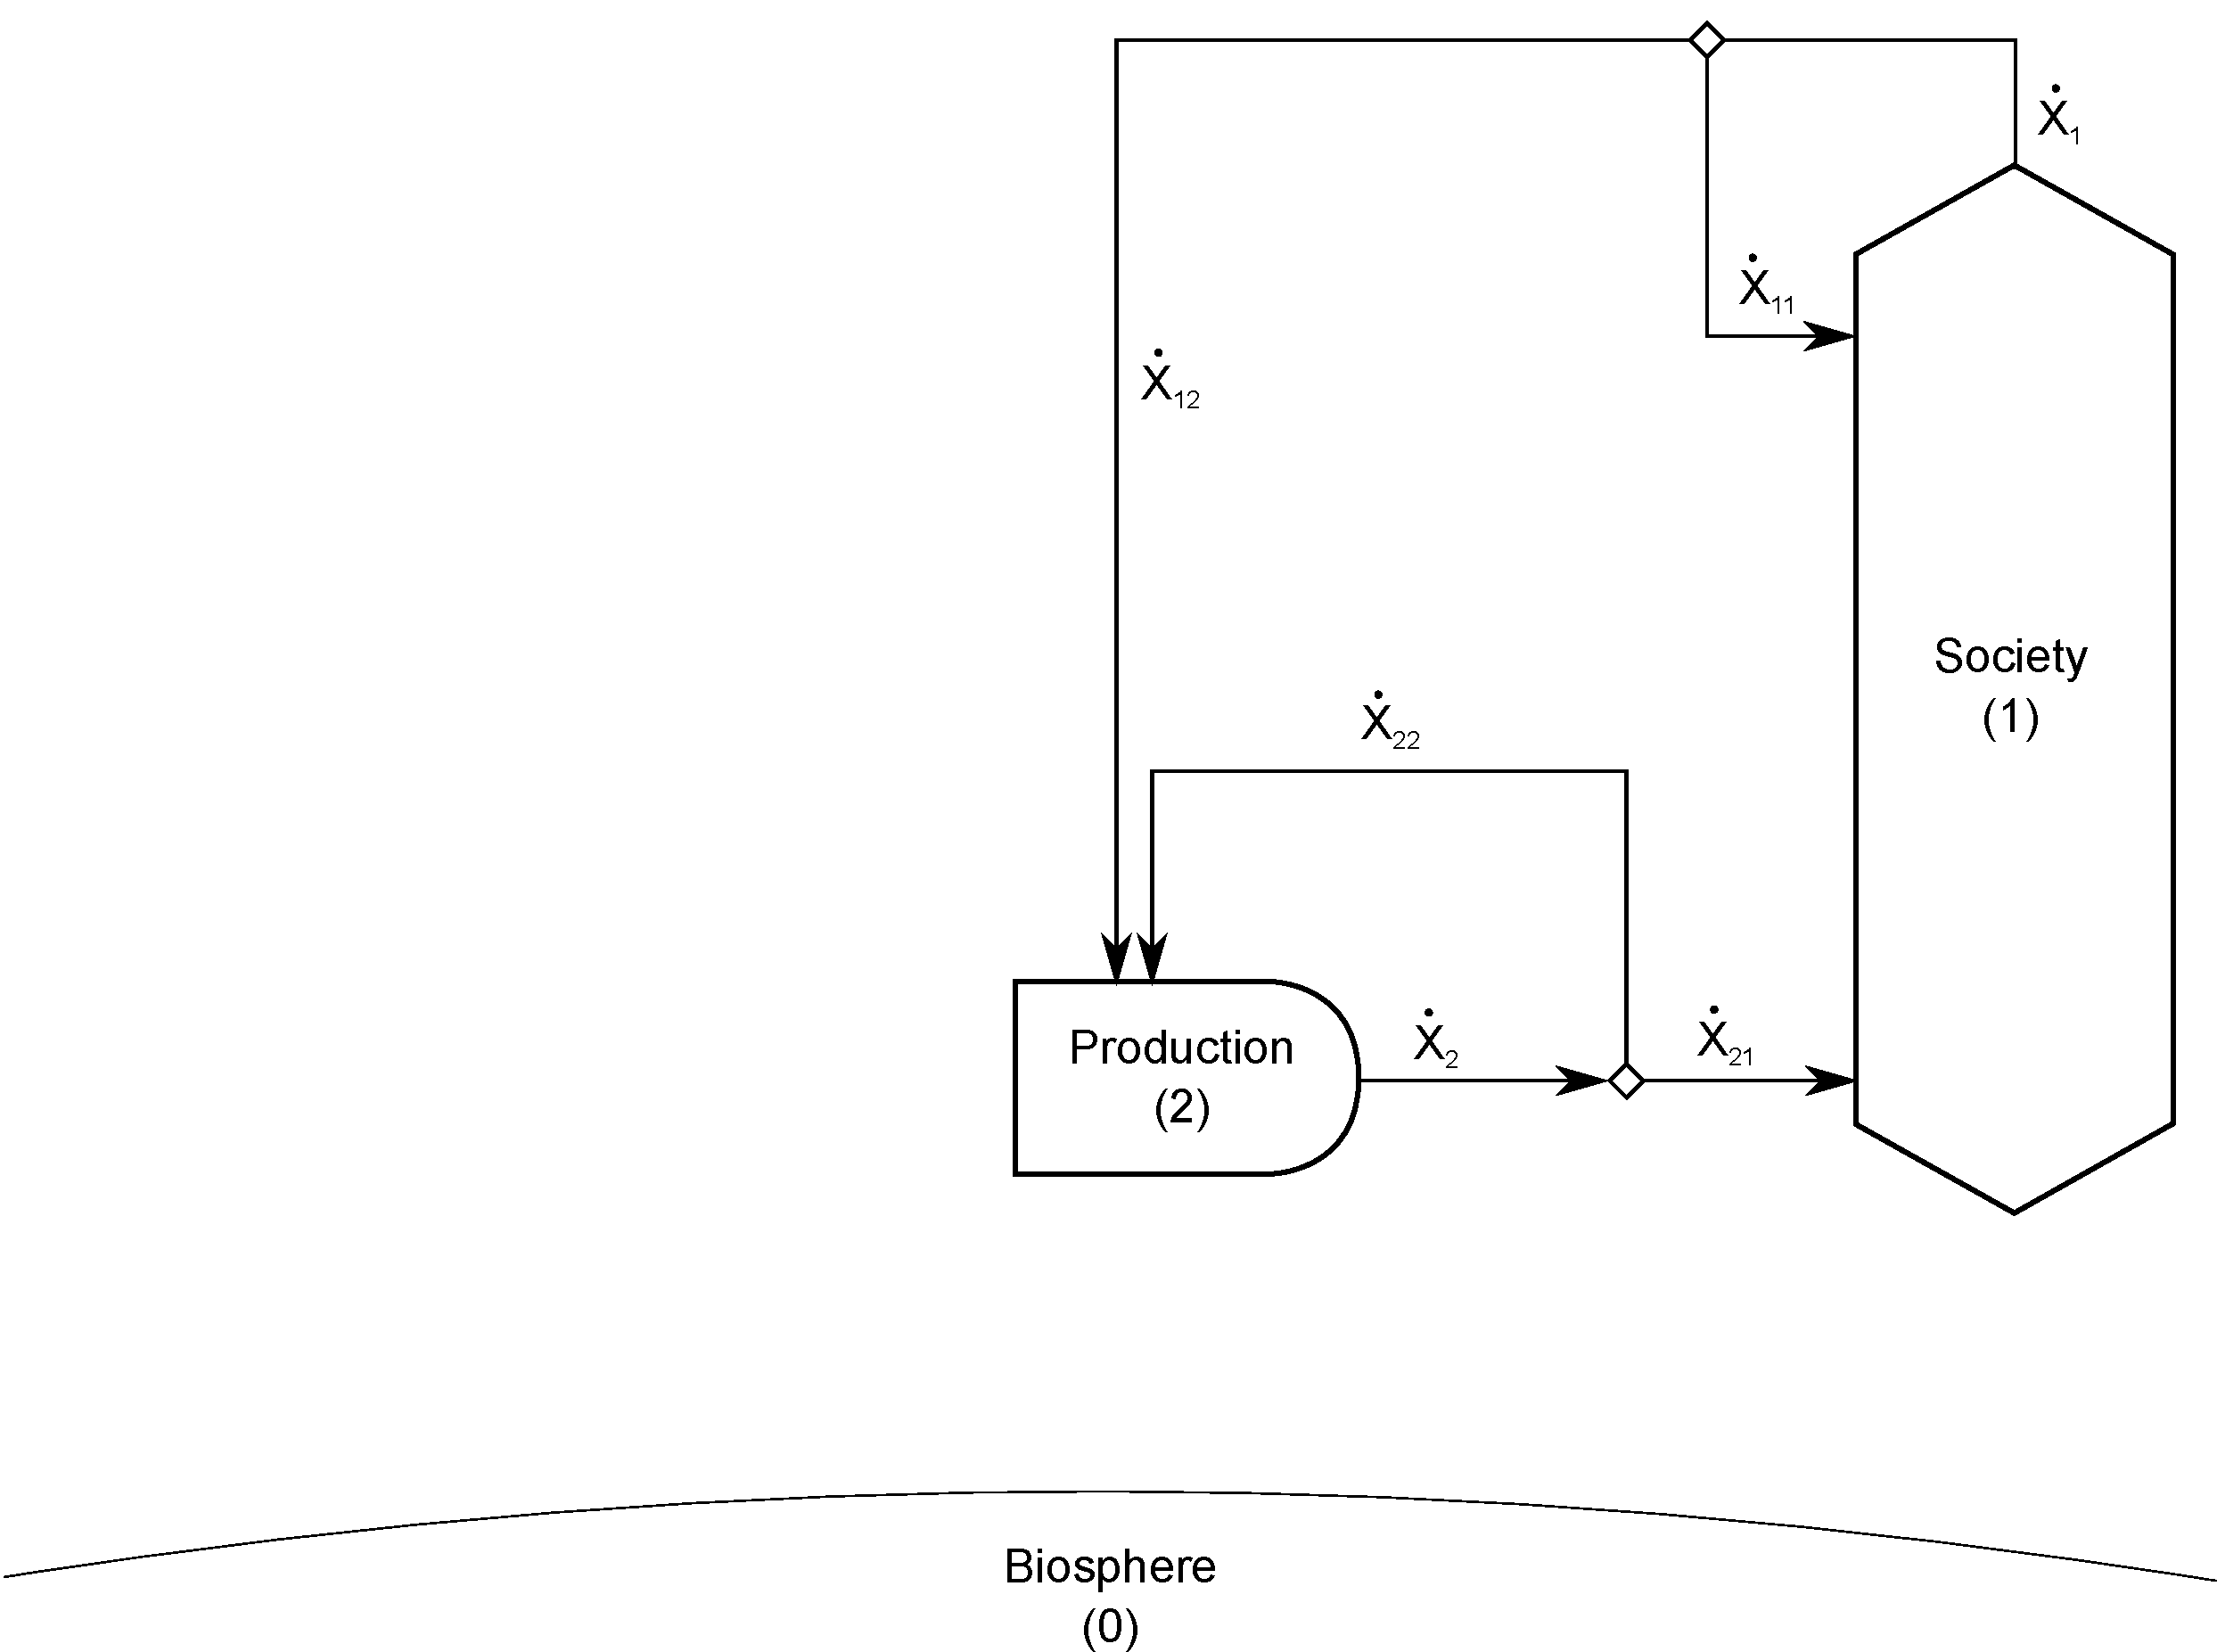
\includegraphics[width=0.8\linewidth]{Part_2/Chapter_Values/images/2_sector_value.pdf}
\caption[Flows of value within a two-sector economy.]{Flows of value ($\dot{X}$) within a two-sector economy.}
\label{fig:B_value}
\end{figure}

We can account for value flows by writing
the following equations:

\begin{equation}\label{eq:B-value-1}
	\frac{\mathrm{d}X_{1}}{\mathrm{d}t}
	= \dot{X}_{11}
	+ \dot{X}_{21}
	- \dot{X}_{1}
	+ \dot{X}_{gen,1}
	- \dot{X}_{dest,1}
\end{equation}

\noindent{}and

\begin{equation}\label{eq:B-value-2}
	\frac{\mathrm{d}X_{2}}{\mathrm{d}t}
	= \dot{X}_{12}
	+ \dot{X}_{22}
	- \dot{X}_{2}
	+ \dot{X}_{gen,2}
	- \dot{X}_{dest,2}.
\end{equation}

Equations~\ref{eq:B-value-1} and~\ref{eq:B-value-2}
can be generalized as

\begin{equation}\label{eq:B-value-generalized}
	\frac{\mathrm{d}X_{j}}{\mathrm{d}t}
	= \sum\limits_{i=1}^n \dot{X}_{ij}
	- \dot{X}_{j}
	+ \dot{X}_{gen,j}
	- \dot{X}_{dest,j},
\end{equation}

\noindent{}where $n$ is the number of sectors in the economy, and $j \in [1, n]$.


%%%%%%%%%% Example C: three-sector economy %%%%%%%%%%
\section{Example C: three-sector economy} % chktex 13
%%%%%%%%%%

Figure~\ref{fig:C_value} shows flows of value ($\dot{X}$) 
within a three-sector economy. 

\begin{figure}[!ht]
\centering
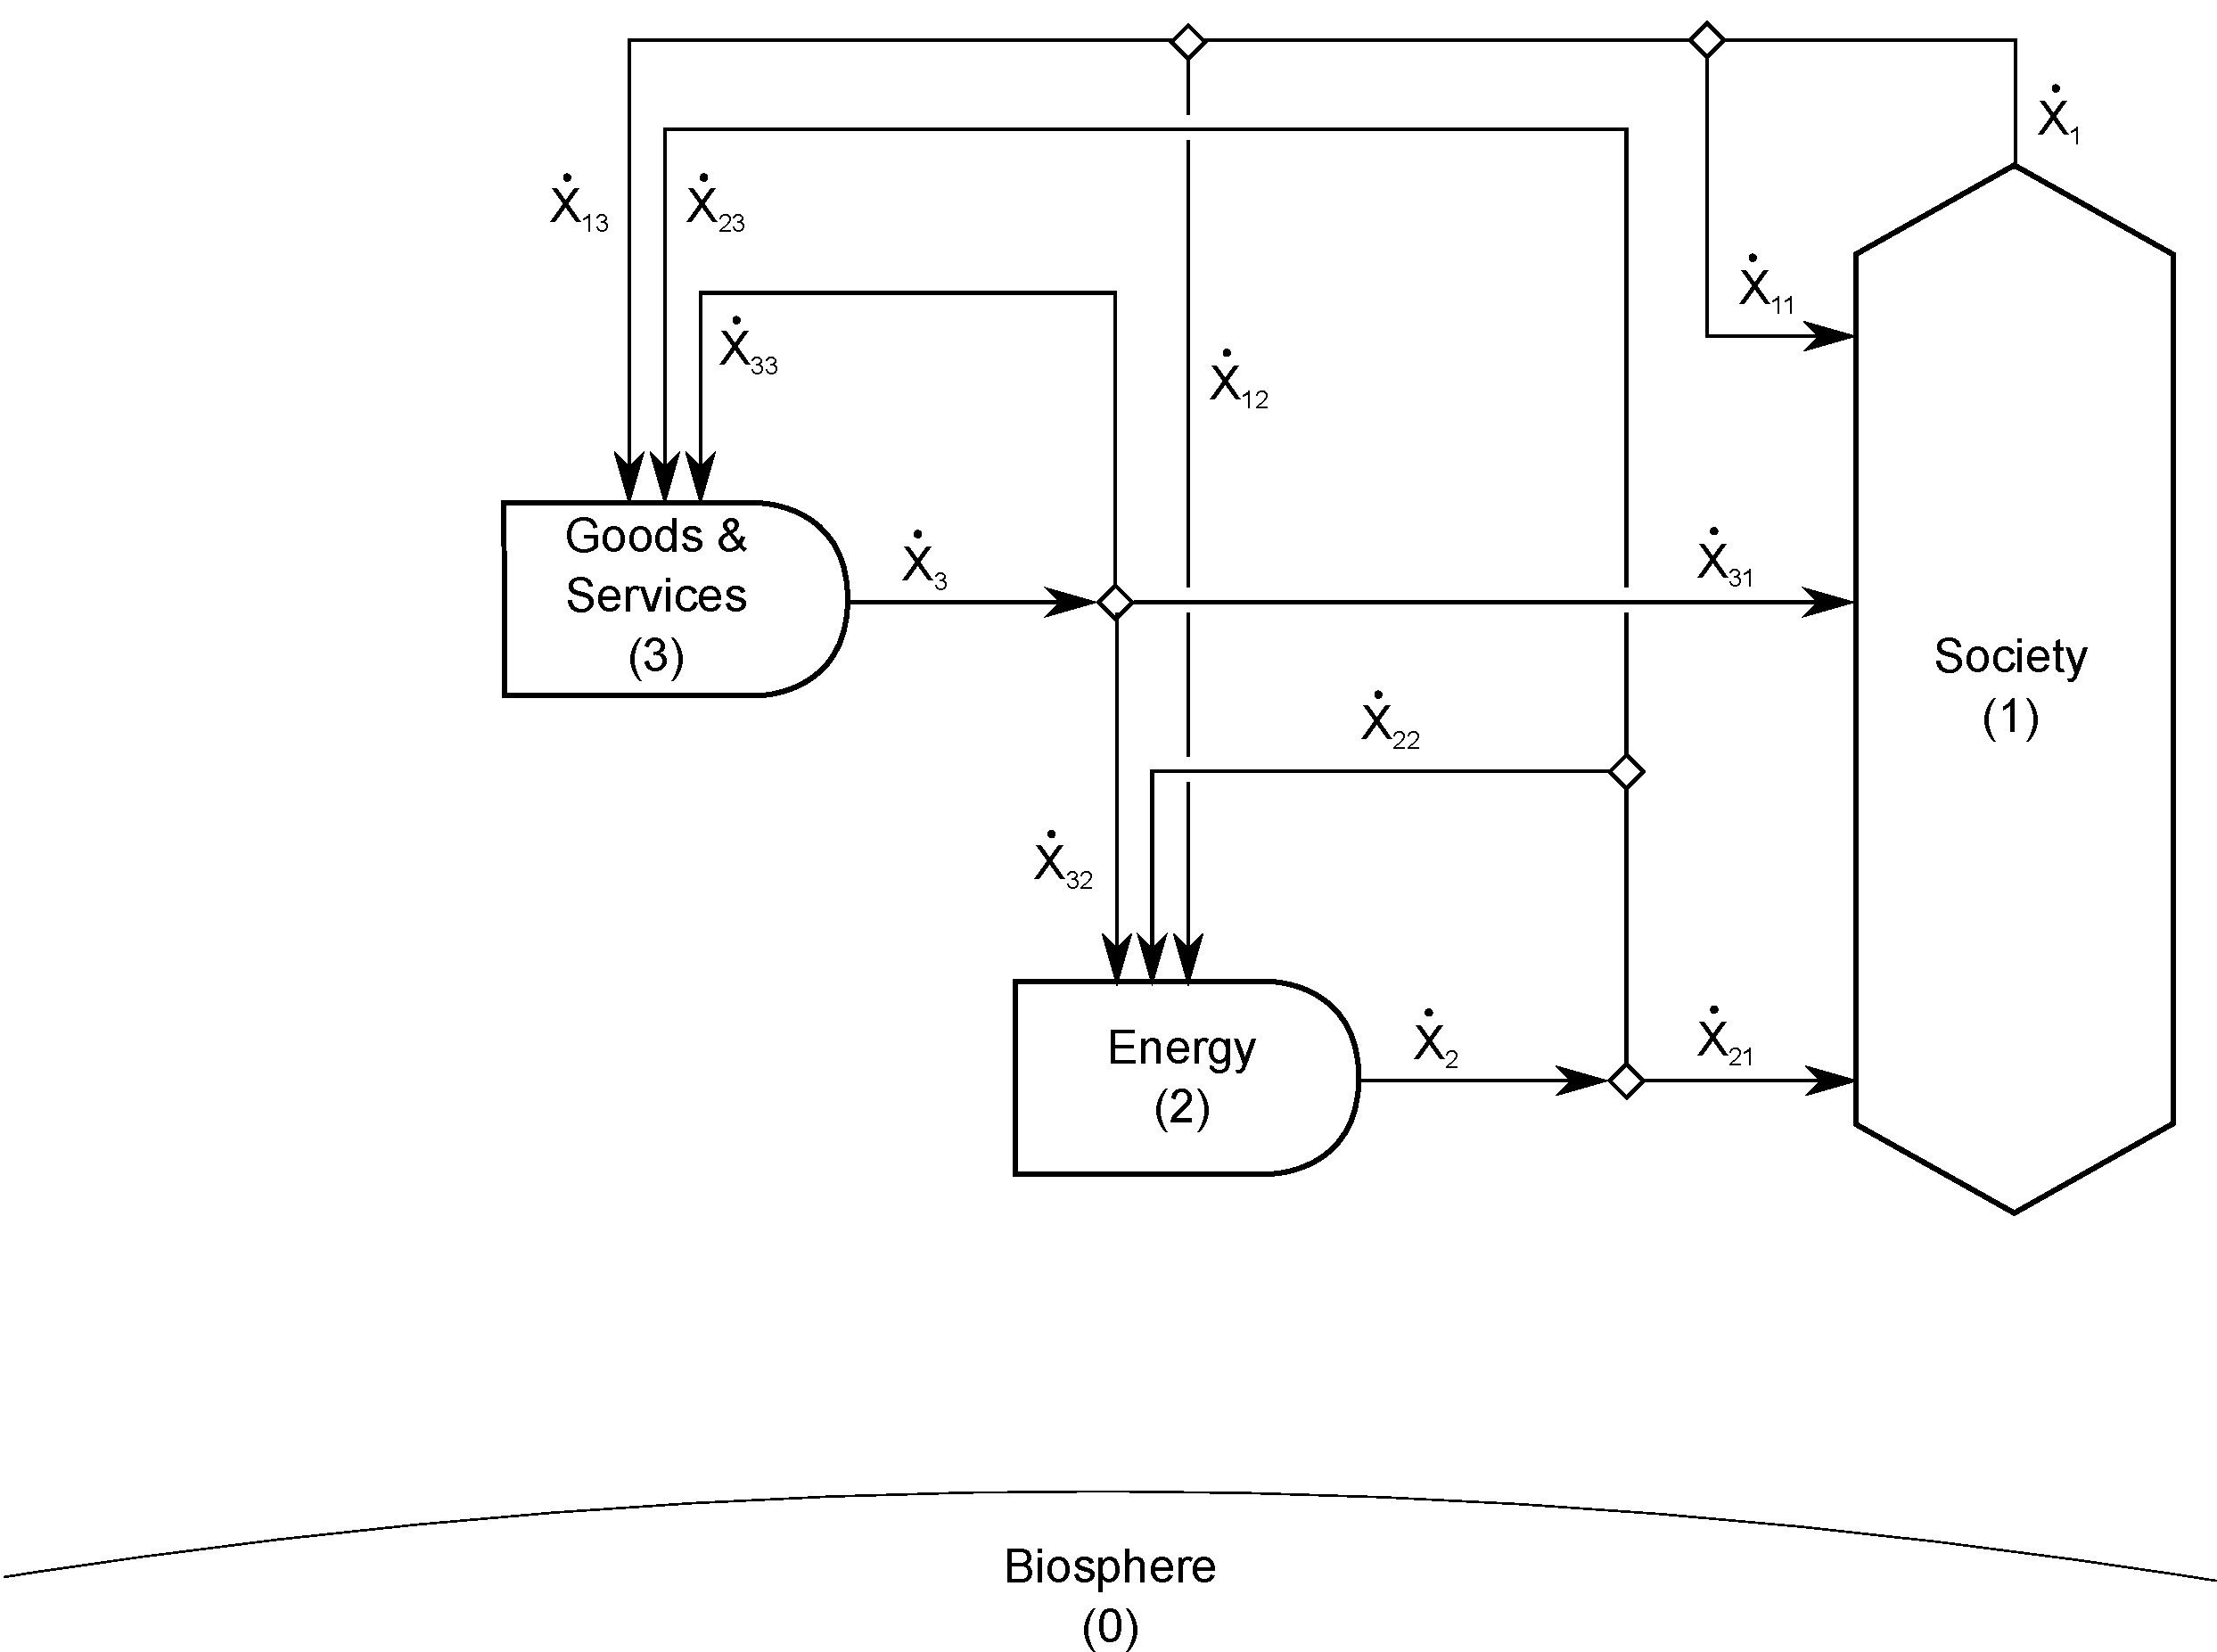
\includegraphics[width=0.8\linewidth]{Part_2/Chapter_Values/images/3_sector_value.pdf}
\caption[Flows of value within a three-sector economy.]{Flows of value ($\dot{X}$) within a three-sector economy.}
\label{fig:C_value}
\end{figure}

The equations representing flows of value in Example~C are:

\begin{equation}\label{eq:C-value-generalized}
	\frac{\mathrm{d}X_{j}}{\mathrm{d}t}
	= \sum\limits_{i=1}^{n} \dot{X}_{ij}
	- \dot{X}_{j}
	+ \dot{X}_{gen,j}
	- \dot{X}_{dest,j},
\end{equation}

\noindent{}where $n$ is the number of sectors in the economy, and $j \in [1, n]$.
Equation~\ref{eq:C-value-generalized} is identical to Equation~\ref{eq:B-value-generalized}.
If we sum the value accounting equations for the entire economy, 
we obtain

\begin{equation}\label{eq:C-value-economy-a}
	\sum\limits_{j=1}^{n} \frac{\mathrm{d}X_{j}}{\mathrm{d}t}
	= \sum\limits_{j=1}^{n} \sum\limits_{i=1}^{n} \dot{X}_{ij}
	- \sum\limits_{j=1}^{n} \dot{X}_{j}
	+ \sum\limits_{j=1}^{n} \dot{X}_{gen,j}
	- \sum\limits_{j=1}^{n} \dot{X}_{dest,j}.
\end{equation}

\noindent{}With the identities

\begin{equation} \label{eq:X_identity_1}
	\dot{X}_{j}  
	= \sum\limits_{k=1}^n \dot{X}_{jk}
\end{equation}

\noindent{}and

\begin{equation} \label{eq:X_identity_2}
	\sum\limits_{j=1}^n\dot{X}_{j}  
	= \sum\limits_{j=1}^n \sum\limits_{k=1}^n \dot{X}_{jk}
	= \sum\limits_{i=1}^n \sum\limits_{k=1}^n \dot{X}_{ik}
	= \sum\limits_{i=1}^n \sum\limits_{j=1}^n \dot{X}_{ij}
	= \sum\limits_{j=1}^n \sum\limits_{i=1}^n \dot{X}_{ij},
\end{equation}

\noindent{}Equation~\ref{eq:C-value-economy-a} becomes

\begin{equation}\label{eq:C-value-economy-b}
	\sum\limits_{j=1}^{n} \frac{\mathrm{d}X_{j}}{\mathrm{d}t}
	= \sum\limits_{j=1}^{n} \dot{X}_{gen,j}
	- \sum\limits_{j=1}^{n} \dot{X}_{dest,j},
\end{equation}

\noindent{}for $j \in [1, n]$, indicating that 
value generation ($\dot{X}_{gen,j}$) 
and destruction ($\dot{X}_{dest,j}$)
are the only mechanisms by which value is accumulated or lost
$\left( \frac{\mathrm{d}X_{j}}{\mathrm{d}t} \right)$
within the economy.


%%%%%%%%%% Value: Auto industry example %%%%%%%%%%
\section{Value in the auto industry}
\label{sec:value_auto}
%%%%%%%%%%

\begin{figure}[!ht]
\centering
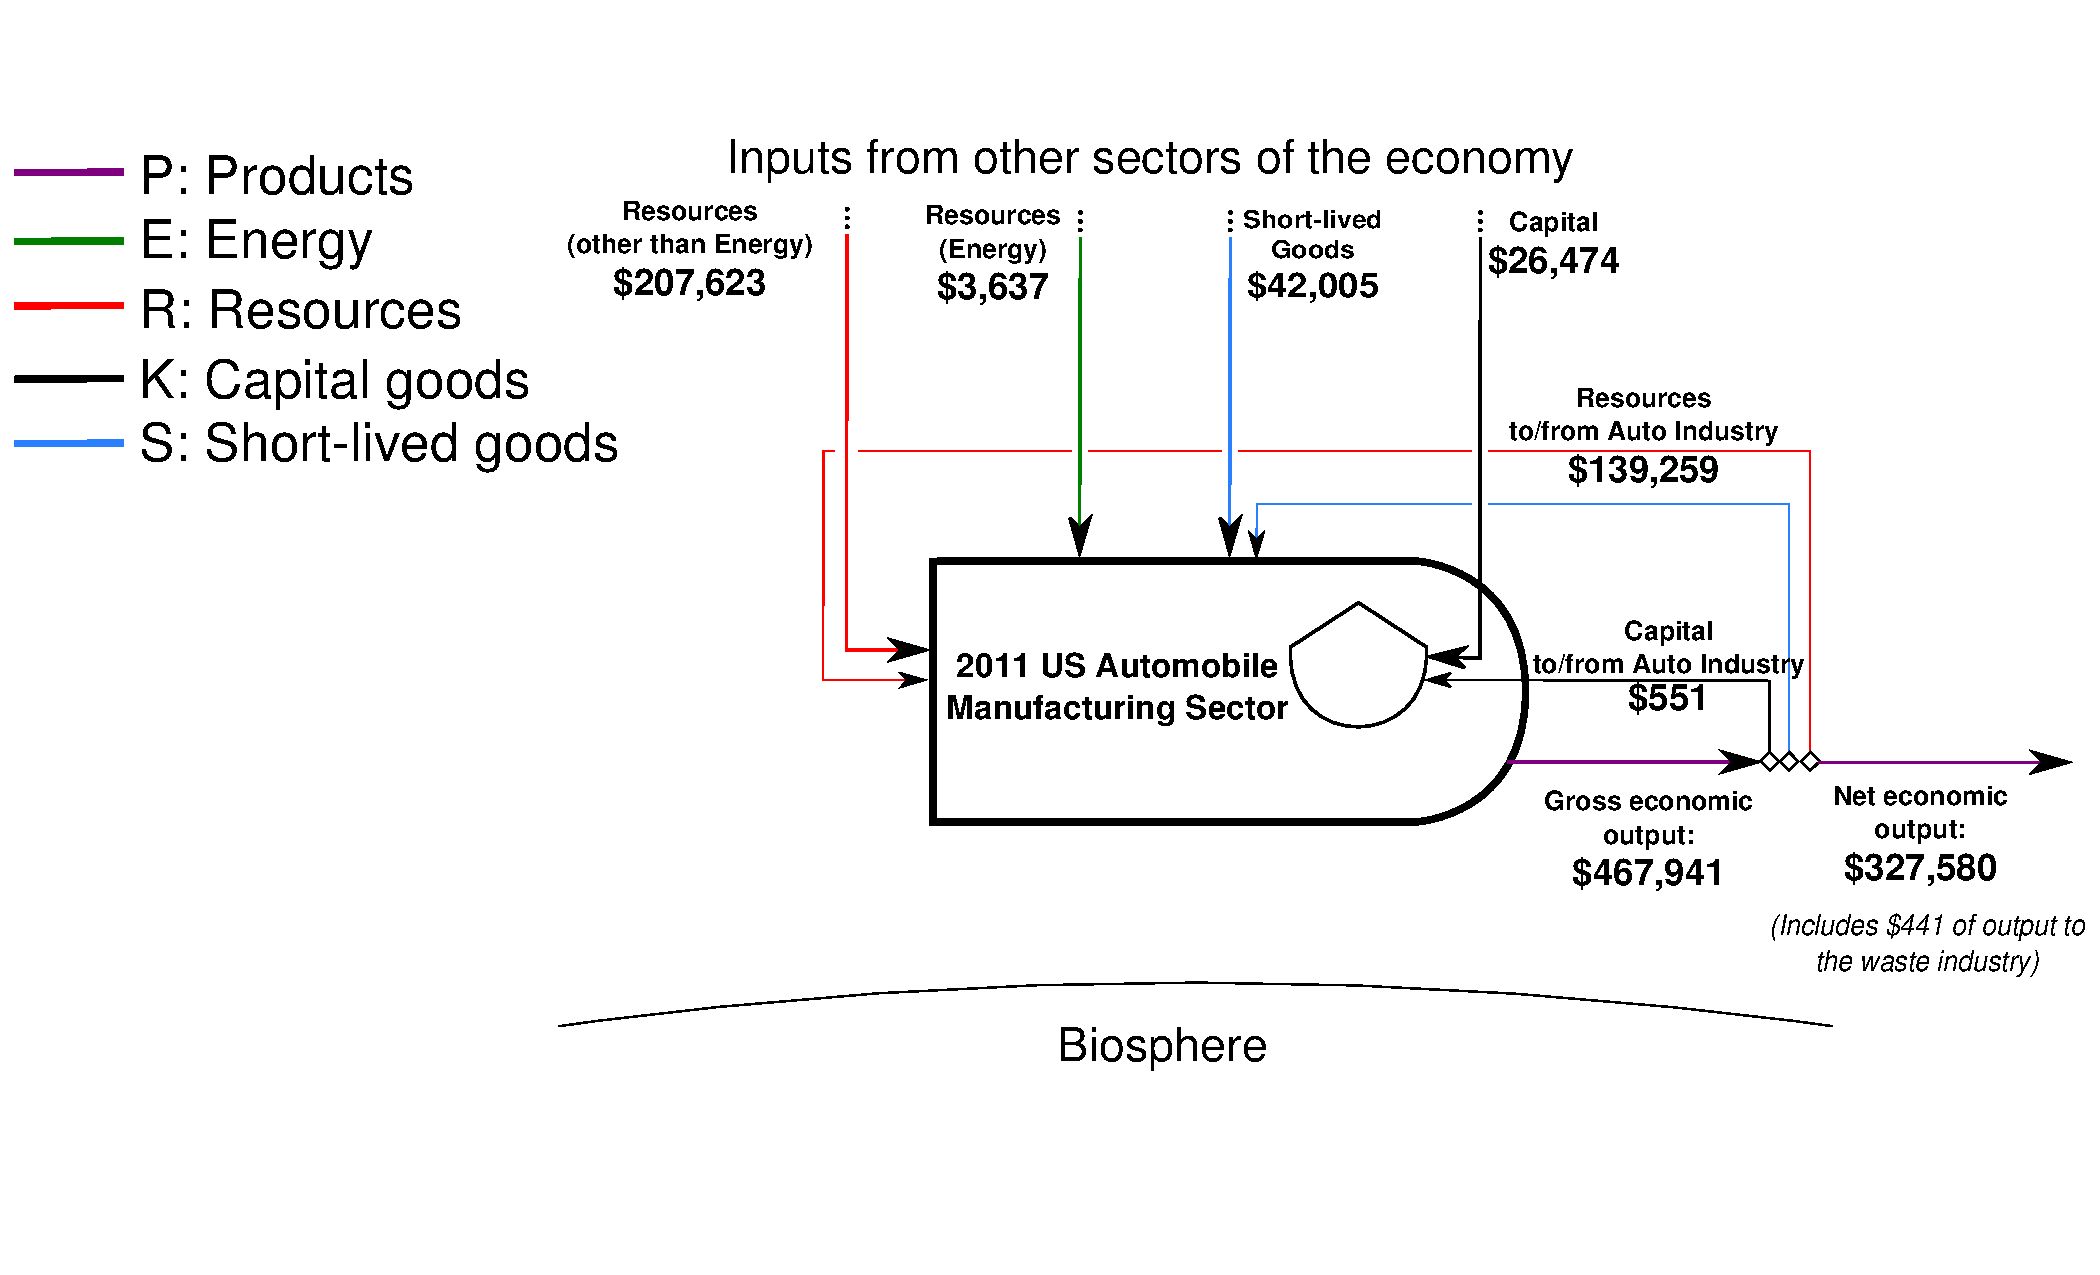
\includegraphics[width=1.0\linewidth]{Part_2/Chapter_Values/images/PERKS_basic_unit_value_auto_ind.pdf}
\caption[Value of Material and Energy flows into and out of the US Automobile Industry]{Value of Material and Energy flows into and out of the US Automobile Industry (2011USD).}
\label{fig:PERKS_value_auto_ind}
\end{figure}


%%%%%%%%%% Value: Summary %%%%%%%%%%
\section{Summary}
\label{sec:value_summary}
%%%%%%%%%%

\bibliographystyle{unsrt}
\bibliography{../../EROI_review_v2}



% Always give a unique label
% and use \ref{<label>} for cross-references
% and \cite{<label>} for bibliographic references
% use \sectionmark{}
% to alter or adjust the section heading in the running head
%% Instead of simply listing headings of different levels we recommend to let every heading be followed by at least a short passage of text. Furtheron please use the \LaTeX\ automatism for all your cross-references and citations.

%% Please note that the first line of text that follows a heading is not indented, whereas the first lines of all sequent paragraphs are.

%% Use the standard \verb|equation| environment to typeset your equations, e.g.
%
%% \begin{equation}
%% a \times b = c\;,
%% \end{equation}
%
%% however, for multiline equations we recommend to use the \verb|eqnarray|
%% environment\footnote{In physics texts please activate the class option \texttt{vecphys} to depict your vectors in \textbf{\itshape boldface-italic} type - as is customary for a wide range of physical jects.}.
%% \begin{eqnarray}
%% a \times b = c \nonumber\\
%% \vec{a} \cdot \vec{b}=\vec{c}
%% \label{eq:01}
%% \end{eqnarray}

%% \section{section Heading}
%% \label{sec:2}
%% Instead of simply listing headings of different levels we recommend to let every heading be followed by at least a short passage of text. Furtheron please use the \LaTeX\ automatism for all your cross-references\index{cross-references} and citations\index{citations} as has already been described in Sect.~\ref{sec:2}.

%% \begin{quotation}
%% Please do not use quotation marks when quoting texts! Simply use the \verb|quotation| environment -- it will automatically render Springer's preferred layout.
%% \end{quotation}


%% \section{section Heading}
%% Instead of simply listing headings of different levels we recommend to let every heading be followed by at least a short passage of text. Furtheron please use the \LaTeX\ automatism for all your cross-references and citations as has already been described in Sect.~\ref{sec:2}, see also Fig.~\ref{fig:1}\footnote{If you copy text passages, figures, or tables from other works, you must obtain \textit{permission} from the copyright holder (usually the original publisher). Please enclose the signed permission with the manucript. The sources\index{permission to print} must be acknowledged either in the captions, as footnotes or in a separate section of the book.}

%% Please note that the first line of text that follows a heading is not indented, whereas the first lines of all sequent paragraphs are.

% For figures use
%
%% \begin{figure}[b]
%% \sidecaption
% Use the relevant command for your figure-insertion program
% to insert the figure file.
% For example, with the option graphics use
%% \includegraphics[scale=.65]{figure}
%
% If not, use
%\picplace{5cm}{2cm} % Give the correct figure height and width in cm
%
%% \caption{If the width of the figure is less than 7.8 cm use the \texttt{sidecapion} command to flush the caption on the left side of the page. If the figure is positioned at the top of the page, align the sidecaption with the top of the figure -- to achieve this you simply need to use the optional argument \texttt{[t]} with the \texttt{sidecaption} command}
%% \label{fig:1}       % Give a unique label
%% \end{figure}


%% \paragraph{Paragraph Heading} %
%% Instead of simply listing headings of different levels we recommend to let every heading be followed by at least a short passage of text. Furtheron please use the \LaTeX\ automatism for all your cross-references and citations as has already been described in Sect.~\ref{sec:2}.

%% Please note that the first line of text that follows a heading is not indented, whereas the first lines of all sequent paragraphs are.

%% For typesetting numbered lists we recommend to use the \verb|enumerate| environment -- it will automatically render Springer's preferred layout.

%% \begin{enumerate}
%% \item{Livelihood and survival mobility are oftentimes coutcomes of uneven socioeconomic development.}
%% \begin{enumerate}
%% \item{Livelihood and survival mobility are oftentimes coutcomes of uneven socioeconomic development.}
%% \item{Livelihood and survival mobility are oftentimes coutcomes of uneven socioeconomic development.}
%% \end{enumerate}
%% \item{Livelihood and survival mobility are oftentimes coutcomes of uneven socioeconomic development.}
%% \end{enumerate}


%% \paragraph{paragraph Heading} In order to avoid simply listing headings of different levels we recommend to let every heading be followed by at least a short passage of text. Use the \LaTeX\ automatism for all your cross-references and citations as has already been described in Sect.~\ref{sec:2}, see also Fig.~\ref{fig:2}.

%% Please note that the first line of text that follows a heading is not indented, whereas the first lines of all sequent paragraphs are.

%% For unnumbered list we recommend to use the \verb|itemize| environment -- it will automatically render Springer's preferred layout.

%% \begin{itemize}
%% \item{Livelihood and survival mobility are oftentimes coutcomes of uneven socioeconomic development, cf. Table~\ref{tab:1}.}
%% \begin{itemize}
%% \item{Livelihood and survival mobility are oftentimes coutcomes of uneven socioeconomic development.}
%% \item{Livelihood and survival mobility are oftentimes coutcomes of uneven socioeconomic development.}
%% \end{itemize}
%% \item{Livelihood and survival mobility are oftentimes coutcomes of uneven socioeconomic development.}
%% \end{itemize}

%% \begin{figure}[t]
%% \sidecaption[t]
% Use the relevant command for your figure-insertion program
% to insert the figure file.
% For example, with the option graphics use
%% \includegraphics[scale=.65]{figure}
%
% If not, use
%\picplace{5cm}{2cm} % Give the correct figure height and width in cm
%
%% \caption{Please write your figure caption here}
%% \label{fig:2}       % Give a unique label
%% \end{figure}

%% \runinhead{Run-in Heading Boldface Version} Use the \LaTeX\ automatism for all your cross-references and citations as has already been described in Sect.~\ref{sec:2}.

%% \runinhead{Run-in Heading Italic Version} Use the \LaTeX\ automatism for all your cross-refer\-ences and citations as has already been described in Sect.~\ref{sec:2}\index{paragraph}.
% Use the \index{} command to code your index words
%
% For tables use
%
%% \begin{table}
%% \caption{Please write your table caption here}
%% \label{tab:1}       % Give a unique label
%
% For LaTeX tables use
%
%% \begin{tabular}{p{2cm}p{2.4cm}p{2cm}p{4.9cm}}
%% \hline\noalign{\smallskip}
%% Classes & class & Length & Action Mechanism  \\
%% \noalign{\smallskip}\svhline\noalign{\smallskip}
%% Translation & mRNA$^a$  & 22 (19--25) & Translation repression, mRNA cleavage\\
%% Translation & mRNA cleavage & 21 & mRNA cleavage\\
%% Translation & mRNA  & 21--22 & mRNA cleavage\\
%%Translation & mRNA  & 24--26 & Histone and DNA Modification\\
%%\noalign{\smallskip}\hline\noalign{\smallskip}
%%\end{tabular}
%%$^a$ Table foot note (with superscript)
%%\end{table}
%
%% \section{Section Heading}
%%\label{sec:3}
% Always give a unique label
% and use \ref{<label>} for cross-references
% and \cite{<label>} for bibliographic references
% use \sectionmark{}
% to alter or adjust the section heading in the running head
%% Instead of simply listing headings of different levels we recommend to let every heading be followed by at least a short passage of text. Furtheron please use the \LaTeX\ automatism for all your cross-references and citations as has already been described in Sect.~\ref{sec:2}.

%% Please note that the first line of text that follows a heading is not indented, whereas the first lines of all sequent paragraphs are.

%%If you want to list definitions or the like we recommend to use the Springer-enhanced \verb|description| environment -- it will automatically render Springer's preferred layout.

%%\begin{description}[Type 1]
%%\item[Type 1]{That addresses central themes pertainng to migration, health, and disease. In Sect.~\ref{sec:1}, Wilson discusses the role of human migration in infectious disease distributions and patterns.}
%%\item[Type 2]{That addresses central themes pertainng to migration, health, and disease. In Sect.~\ref{sec:2}, Wilson discusses the role of human migration in infectious disease distributions and patterns.}
%%\end{description}

%%\section{section Heading} %
%% In order to avoid simply listing headings of different levels we recommend to let every heading be followed by at least a short passage of text. Use the \LaTeX\ automatism for all your cross-references and citations citations as has already been described in Sect.~\ref{sec:2}.

%% Please note that the first line of text that follows a heading is not indented, whereas the first lines of all sequent paragraphs are.

%% \begin{svgraybox}
%% If you want to emphasize complete paragraphs of texts we recommend to use the newly defined Springer class option \verb|graybox| and the newly defined environment \verb|svgraybox|. This will produce a 15 percent screened box 'behind' your text.

%% If you want to emphasize complete paragraphs of texts we recommend to use the newly defined Springer class option and environment \verb|svgraybox|. This will produce a 15 percent screened box 'behind' your text.
%% \end{svgraybox}


%% \section{section Heading}
%%Instead of simply listing headings of different levels we recommend to let every heading be followed by at least a short passage of text. Furtheron please use the \LaTeX\ automatism for all your cross-references and citations as has already been described in Sect.~\ref{sec:2}.

%% Please note that the first line of text that follows a heading is not indented, whereas the first lines of all sequent paragraphs are.

%% \begin{theorem}
%% Theorem text goes here.
%% \end{theorem}
%
% or
%
%% \begin{definition}
%% Definition text goes here.
%% \end{definition}

%% \begin{proof}
%\smartqed
%% Proof text goes here.
%% \qed
%% \end{proof}

%%\paragraph{Paragraph Heading} %
%% Instead of simply listing headings of different levels we recommend to let every heading be followed by at least a short passage of text. Furtheron please use the \LaTeX\ automatism for all your cross-references and citations as has already been described in Sect.~\ref{sec:2}.

%% Note that the first line of text that follows a heading is not indented, whereas the first lines of all subsequent paragraphs are.
%
% For built-in environments use
%
%%\begin{theorem}
%%Theorem text goes here.
%%\end{theorem}
%
%%\begin{definition}
%%Definition text goes here.
%%\end{definition}
%
%%\begin{proof}
%%\smartqed
%% Proof text goes here.
%%\qed
%%\end{proof}
%
%% \begin{acknowledgement}
%% If you want to include acknowledgments of assistance and the like at the end of an individual chapter please use the \verb|acknowledgement| environment -- it will automatically render Springer's preferred layout.
%% \end{acknowledgement}
%
%% \section*{Appendix}
%% \addcontentsline{toc}{section}{Appendix}
%
%% When placed at the end of a chapter or contribution (as opposed to at the end of the book), the numbering of tables, figures, and equations in the appendix section continues on from that in the main text. Hence please \textit{do not} use the \verb|appendix| command when writing an appendix at the end of your chapter or contribution. If there is only one the appendix is designated ``Appendix'', or ``Appendix 1'', or ``Appendix 2'', etc. if there is more than one.

%% \begin{equation}
%% a \times b = c
%% \end{equation}
% Problems or Exercises should be sorted chapterwise
%% \section*{Problems}
%% \addcontentsline{toc}{section}{Problems}
%
% Use the following environment.
% Don't forget to label each problem;
% the label is needed for the solutions' environment
%% \begin{prob}
%% \label{prob1}
%% A given problem or Excercise is described here. The
%% problem is described here. The problem is described here.
%% \end{prob}

%% \begin{prob}
%% \label{prob2}
%% \textbf{Problem Heading}\\
%% (a) The first part of the problem is described here.\\
%% (b) The second part of the problem is described here.
%% \end{prob}


